\documentclass{standalone}
\usepackage{tikz}
\begin{document}
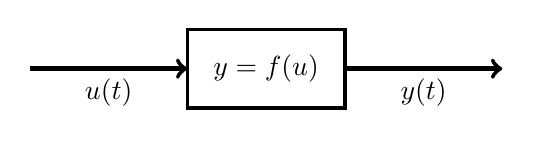
\begin{tikzpicture}[scale=2]
    \node[rectangle, draw, very thick, minimum width=2cm, minimum height=1cm](r)at(0,0){$y=f(u)$};

    \draw[->,ultra thick](-1.5,0)--(-0.5,0);
    \node[below]at(-1,0){$u(t)$};

    \draw[<-,ultra thick](1.5,0)--(0.5,0);
    \node[below]at(1,0){$y(t)$};
\end{tikzpicture}
\end{document}